\documentclass[11pt]{article}

\usepackage[a4paper,margin=2.6cm]{geometry}
\usepackage[T1]{fontenc}
\usepackage[utf8]{inputenc}
\usepackage{lmodern}
\usepackage{microtype}
\usepackage{amsmath,amssymb,mathtools}
\usepackage{booktabs}
\usepackage{array}
\usepackage{enumitem}
\usepackage{graphicx}
\usepackage{tikz}
\usetikzlibrary{arrows.meta,positioning,fit}
\usepackage[backend=biber,style=authoryear,natbib=true,maxcitenames=2,maxbibnames=99]{biblatex}
\addbibresource{references.bib}
\usepackage[hidelinks]{hyperref}
\usepackage[nameinlink,noabbrev]{cleveref}
\emergencystretch=2em

\newcommand{\Prob}{\mathbb{P}}
\newcommand{\E}{\mathbb{E}}
\newcommand{\R}{\mathbb{R}}
\newcommand{\calO}{\mathcal{O}}
\newcommand{\calS}{\mathcal{S}}
\newcommand{\calC}{\mathcal{C}}
\newcommand{\method}{\textsc{FAMS}}

\title{Failure-Aware Multimodal Behavioural Sensing:\\
Probabilistic State Inference, Person Attribution, and Sensor Reduction in Smart Homes}
\author{Diogo Ribeiro\\
\small \textit{Faculty of Media Arts and Design, Technical University of Porto}}
\date{}

\begin{document}
\maketitle

\begin{abstract}
Ambient assisted-living systems typically infer human behaviour from sparse, heterogeneous, and imperfect sensor streams. A recurring methodological weakness is that sensor activation is treated too directly as behavioural truth: an object interaction is interpreted as an activity, silence is interpreted as inactivity, and all ambient events are implicitly attributed to the monitored resident. We present a failure-aware multimodal framework that instead represents sensor events as uncertain observations of latent behavioural state. The framework combines a hardware-neutral observation model, online sensor-health estimation, probabilistic occupancy and resident attribution, continuous-time latent-state filtering, adaptive personal baselines, restrained alerting, and paired sensor-ablation experiments. Missing or failed sensors are represented as missing evidence rather than negative evidence, and the inference layer is designed to abstain when coverage or posterior separation is insufficient. A synthetic household generator, deliberately structurally distinct from the estimator, provides controlled ground truth for stress testing sensor failure, visitor contamination, wearable non-adherence, asynchronous observations, and behavioural change. Exploratory simulator-only results indicate that the framework degrades gradually under missing observations, that occupancy-aware attribution is most useful when another person is present, and that reduced multimodal deployments can approach the state-inference performance of larger object-sensor configurations. These numbers are not estimates of field performance. Development-stage evaluation on 22 real annotated homes shows why: median balanced accuracy falls to 0.420, a supervised classifier given the same sensor information reaches only 0.607, so the simulator represents an easier problem than the instrumentation supports for any method; and the abstention mechanism did not function, its stated confidence separating correct from incorrect answers by 0.073 and inverting above 0.95. We therefore define a pre-specified confirmatory simulation study and a frozen external-validation protocol on annotated public smart-home datasets. The contribution is methodological: an architecture in which whether the evidence suffices, and which sensors carry non-redundant information, are answerable questions rather than assumptions.
\end{abstract}

\noindent\textbf{Keywords:} ambient assisted living; behavioural sensing; sensor fusion; uncertainty; smart homes; missing data; multi-resident activity recognition; change detection; sensor ablation

\section{Introduction}

Ambient assisted living (AAL) offers a route to continuous, low-burden monitoring in the home, but the useful signal is indirect. Motion detectors, contact switches, bed sensors, wearables, and radar systems measure physical phenomena; they do not directly observe activities of daily living, health states, or clinical deterioration. Recent reviews accordingly describe AAL design as a system-level trade-off between sensing quality, privacy, usability, reliability, communication, cost, and decision-making \citep{zieni2025aal}. Statistical work on passive sensing has shown that interpretable models can capture within-home temporal structure and cross-sensor dependence \citep{gillam2022athome}, while smart-home activity recognition has developed increasingly sophisticated sequential and multi-person models \citep{asghari2019hhmm,wang2022multiperson}. Four problems remain acute for longitudinal monitoring.

First, \emph{sensor semantics are often stronger than the evidence}. A refrigerator-door activation is evidence of kitchen or object interaction, not proof that food was consumed. A tap activation is not direct measurement of hydration. A bed-pressure state is not polysomnographic sleep. Treating proxy sensors as behavioural labels creates a semantic error before any statistical model is fitted.

Second, \emph{missingness and failure are behaviourally confounded}. A quiet event stream may indicate inactivity, a changed routine, packet loss, battery degradation, gateway failure, or an uninstalled sensor. If missing records are silently represented as zeros, inference can become confidently wrong in the direction of reduced activity. Deterioration and sensor under-delivery then produce superficially similar data, which is precisely the discrimination longitudinal monitoring needs to make.

Third, \emph{activity in the home is not necessarily activity by the monitored resident}. Multi-resident activity recognition is a known hard problem \citep{wang2022multiperson,alemdar2013aras}. Visitors and carers can trigger the same ambient sensors used to construct behavioural summaries. A single-resident model therefore needs either explicit attribution or explicit uncertainty about attribution.

Fourth, \emph{more sensors are not automatically better}. Additional sensors increase installation burden, maintenance, cost, failure surfaces, and potentially privacy risk. Emerging privacy-preserving modalities such as millimetre-wave radar can provide richer presence, motion, posture, and tracking information without cameras \citep{chen2026mmwave,samimi2026fmcw}. The design question is therefore which sensor subsets retain useful information and remain robust when components fail, not which model scores best on a fixed deployment.

We address these issues through an uncertainty-aware research framework for multimodal behavioural sensing. The framework is deliberately interpretable and modular. Its central quantity is a posterior distribution over latent behavioural states,
\begin{equation}
    \Prob(Z_t=z\mid \calO_{1:t}),
\end{equation}
where $Z_t$ denotes a latent behavioural state and $\calO_{1:t}$ is the heterogeneous observation history. Sensor quality, sensor-health reliability, and resident attribution temper the evidential contribution of each observation. A failed sensor contributes no state preference; it does not vote for inactivity.

The paper makes five methodological contributions:
\begin{enumerate}[label=(\roman*)]
    \item a canonical observation model that separates physical measurement from behavioural interpretation;
    \item reliability-aware multimodal filtering with explicit abstention and evidence-level explanations;
    \item occupancy-aware resident attribution for visitor and carer contamination;
    \item adaptive personal baselines that separate ordinary variability, drift, abrupt change, and poor observation quality; and
    \item a paired sensor-ablation design for estimating marginal and interaction effects of sensing modalities.
\end{enumerate}

Contribution (ii) is the one this manuscript is least able to support. The
abstention mechanism is specified and implemented, but every measurement we have
of whether it works is negative, and the two failures are of different kinds. On
real recordings it abstained on 2.2\% of steps while its confidence carried
almost no information about correctness (\cref{sec:abstentionfailure}). In the
frozen confirmatory simulation of \cref{sec:confirmatory-results} it barely
abstained at all:
mean abstention rose only from $9.7\times10^{-6}$ to $5.3\times10^{-5}$ as
random missingness went from 0\% to 40\%, so discarding two fifths of the
evidence left the mechanism essentially silent. We therefore report (ii) as an
architectural contribution and as a negative result about the formulation.

\paragraph{Evidence status.}
This manuscript reports results at two evidential levels, and they should not be
read as interchangeable. The simulator results in \cref{sec:pilotresults} are
exploratory: they come from a project-authored generator and document the
behaviour of the implementation rather than estimating field performance. The
results in \cref{sec:realdev} come from 22 real annotated homes, which removes
the circularity but not the selection: those recordings were inspected
repeatedly while diagnosing failure modes, so they are development evidence and
not a held-out test. Neither level supports a claim about deployment
performance.

The other two levels are confirmatory, and were frozen before execution. The
simulation study of \cref{sec:confirmatory-results} was run once under the
protocol in \cref{sec:confirmatory}; its outcomes are simulator-derived and
estimate nothing about field performance. The external validation of
\cref{sec:external} was scored once against a cohort of homes frozen before any
outcome was seen, and is the only result here that is confirmatory on real
data. Where the four levels disagree, the weaker one does not soften the
stronger.

\section{Related work}

\subsection{Passive and ambient sensing}

Passive sensing has long been attractive for home monitoring because it can observe routine without requiring repeated user interaction. \citet{gillam2022athome} modelled passive home-sensor activations as binary time series with autoregressive and cross-sensor structure, demonstrating the value of transparent household-specific probabilistic models. More broadly, AAL systems now combine ambient, wearable, environmental, and increasingly radar-based sensing, but system reliability and privacy remain central constraints \citep{zieni2025aal}.

Sequential latent-state models are natural for activity recognition because activities exhibit persistence and transitions. Hierarchical hidden Markov models have been proposed for online activity recognition in smart environments \citep{asghari2019hhmm}. Change-point detection provides a complementary view by focusing on transitions rather than labels; it has been used both for smart-home activity segmentation \citep{bermejo2021cpd} and energy-efficient wearable monitoring \citep{culman2020cpam}. Our framework retains this statistical tradition but places observation quality, failure state, and person attribution directly in the inference chain.

\subsection{Multiple residents and attribution}

The association between an ambient sensor event and the person who generated it is a separate inference problem from recognising the activity itself. ARAS provides multi-resident smart-home data collected in two real homes with 20 binary sensors and 27 activities \citep{alemdar2013aras}. \citet{wang2022multiperson} showed that jointly estimating resident count and associating observations with residents can materially improve multi-person activity recognition. Our scope is narrower: we model one monitored resident and treat other occupants as contextual contamination rather than attempting biometric identity or complete multi-resident state tracking. This allows attribution uncertainty to be propagated without cameras, microphones, or facial recognition.

\subsection{Richer privacy-preserving sensing}

Millimetre-wave radar is increasingly relevant to AAL because it can provide contactless presence, motion, tracking, posture, and vital-sign features without optical imagery. Recent work has demonstrated multi-person fall detection in realistic indoor environments \citep{chen2026mmwave} and human activity recognition using 60~GHz FMCW radar \citep{samimi2026fmcw}. We treat radar as one modality among several and consume derived probabilistic features rather than raw radar cubes. The methodological question is whether such information-rich modalities can replace several narrow object sensors without making the inference less calibrated or less robust.

\section{Methodological framework}
\label{sec:method}

\begin{figure}[t]
\centering
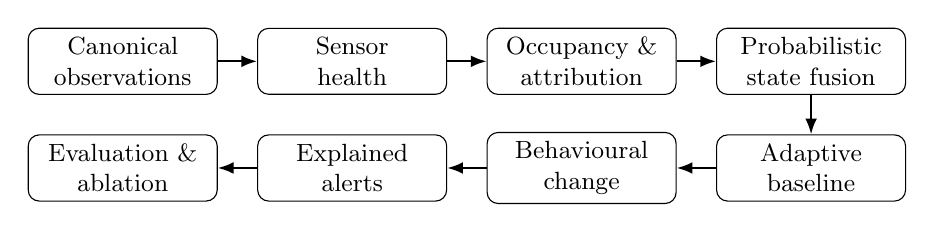
\begin{tikzpicture}[
  node distance=5mm and 5mm,
  box/.style={draw, rounded corners, align=center, minimum height=8mm, minimum width=24mm, font=\small},
  arr/.style={-{Latex[length=2mm]}, thick}
]
\node[box] (obs) {Canonical\\observations};
\node[box, right=of obs] (health) {Sensor\\health};
\node[box, right=of health] (context) {Occupancy \&\\attribution};
\node[box, right=of context] (fusion) {Probabilistic\\state fusion};
\node[box, below=of fusion] (baseline) {Adaptive\\baseline};
\node[box, left=of baseline] (change) {Behavioural\\change};
\node[box, left=of change] (alerts) {Explained\\alerts};
\node[box, left=of alerts] (eval) {Evaluation \&\\ablation};
\draw[arr] (obs) -- (health);
\draw[arr] (health) -- (context);
\draw[arr] (context) -- (fusion);
\draw[arr] (fusion) -- (baseline);
\draw[arr] (baseline) -- (change);
\draw[arr] (change) -- (alerts);
\draw[arr] (alerts) -- (eval);
\end{tikzpicture}
\caption{Conceptual processing chain. The separation between observation, health, attribution, state inference, change, and alert is deliberate: each layer answers a different question and carries its uncertainty forward.}
\label{fig:architecture}
\end{figure}

\subsection{Canonical observations and temporal semantics}

A sensor observation is represented abstractly as
\begin{equation}
O_i = (t_i,s_i,m_i,k_i,x_i,u_i,q_i,c_i,\rho_i),
\end{equation}
where $t_i$ is a timezone-aware timestamp, $s_i$ a sensor identifier, $m_i$ the modality, $k_i$ the temporal kind, $x_i$ the value, $u_i$ its unit, $q_i\in[0,1]$ a device-quality measure, $c_i\in[0,1]$ confidence in a derived value, and $\rho_i$ provenance/context metadata.

The temporal kind is essential. We distinguish:
\begin{itemize}
    \item \textbf{events}: instantaneous occurrences; an absent record is not a measured zero;
    \item \textbf{states}: levels that persist until changed, with bounded carry-forward; and
    \item \textbf{samples}: measurements of continuously existing quantities, where an absent record means unobserved.
\end{itemize}
It prevents forward-filling an event stream, and prevents communication failure from being recorded as a sequence of behavioural zeros.

The semantic boundary is similarly explicit. A sensor can support a state such as \emph{kitchen activity}; it cannot by itself establish \emph{food consumption}. Higher-level interpretations require additional evidence and should retain uncertainty.

\subsection{Sensor health as evidential reliability}

For sensor $s$ at time $t$, the health layer estimates a reliability weight
\begin{equation}
    r_s(t)\in[0,1].
\end{equation}
Statuses include healthy, degraded, drifting, out-of-range, stuck, dropout, missing, and unknown. Reliability depends on declared reporting semantics. Silence from a purely event-driven contact sensor cannot by itself diagnose failure, whereas a sampled sensor that promised a one-minute cadence can be judged against that promise.

The governing rule is
\begin{equation}
    r_s(t)=0 \quad \Longrightarrow \quad
    \text{sensor $s$ contributes no state preference}.
\end{equation}
A missing sensor supplies missing evidence, not evidence for a low-activity state. Partial under-delivery is detectable for sensors with a declared cadence; for event-only sensors without a heartbeat, behavioural quiet and transport loss remain fundamentally confounded.

\subsection{Occupancy context and resident attribution}

Let $C_t\in\calC$ denote an occupancy context, for example resident alone, resident with visitor, visitor only, or uncertain occupancy. The context layer maintains
\begin{equation}
    \Prob(C_t=c\mid \calO_{1:t})
\end{equation}
and derives an attribution factor for each ambient sensor,
\begin{equation}
    a_s(t)=\Prob(\text{resident generated evidence from $s$}\mid\calO_{1:t}).
\end{equation}
Person-bound sensing, such as a worn device or resident beacon, can remain fully attributable when valid. Ambient evidence is discounted when the monitored resident may not be its source. The framework does not attempt biometric identity; it represents uncertainty about authorship.

\subsection{Continuous-time multimodal state inference}

Let $Z_t\in\calS$ be a latent behavioural state. A configurable ontology may contain states such as away, home-active, home-inactive, sleeping, bed-awake, bathroom-activity, kitchen-activity, and an external abstention state \texttt{UNKNOWN}. The latter is not part of the Markov state vector; it is emitted only when inference is insufficient.

Between observations, the belief evolves under a continuous-time Markov generator $Q$:
\begin{equation}
    \boldsymbol{p}(t+\Delta)
    = \boldsymbol{p}(t)\exp(Q\Delta).
\end{equation}
For a batch of observations $B_t$, each sensor supplies a likelihood contribution $L_s(z)$. We use a tempered update
\begin{equation}
    p_t(z)
    \propto
    p_{t^-}(z)
    \prod_{s\in B_t} L_s(z)^{\omega_s(t)},
\end{equation}
with
\begin{equation}
    \omega_s(t)=\lambda_s\,q_s(t)c_s(t)r_s(t)a_s(t),
\end{equation}
where $\lambda_s$ is a declared modality/evidence weight. Power-likelihood tempering provides a smooth way to reduce the contribution of uncertain evidence; at zero weight the likelihood becomes flat. This is closely related to general Bayesian updating, in which information can be connected to belief through a loss or tempered likelihood rather than an assumed perfectly specified global data-generating model \citep{bissiri2016general}.

The filter exposes the full posterior, leading-state confidence, entropy, margin, completeness, supporting evidence, contradictory evidence, silent-but-working sensors, and missing sensors. It abstains when either confidence or sensor completeness falls below a pre-specified threshold.

\subsection{Adaptive personal baselines}

Daily behavioural summaries are integrated from posterior state occupancy rather than argmax labels. For state $z$ on day $d$,
\begin{equation}
    H_{d,z}=\sum_{t\in d} p_t(z)\,\Delta t.
\end{equation}
Poorly observed days are excluded from baseline learning. For a daily feature $X_d$, a robust deviation score can be written as
\begin{equation}
    D_d =
    \frac{X_d-\widetilde{\mu}_d}
    {\max\{1.4826\,\operatorname{MAD}_d,\epsilon\}},
\end{equation}
where the reference may be weekday-aware. Change-point methods complement this local deviation view by separating persistent shifts from ordinary day-to-day noise; PELT and related methods are well suited to this role \citep{killick2012pelt}. The baseline is adaptive but is not allowed to learn indiscriminately from low-coverage days.

\subsection{Behavioural change and alerts}

Observation, state, change, and alert are distinct objects. A statistically unusual day does not automatically trigger a delivered alert. Alerting may depend on magnitude, duration, persistence, confidence, attribution, sensor health, and deduplication/rate-limiting. This distinction is required to evaluate the quantity a recipient experiences: false alerts per person-day, rather than only algorithmic threshold crossings.

\subsection{Sensor ablation and interaction}

Let $S\subseteq\calS_{\mathrm{sens}}$ denote a deployment sensor set and $M(S)$ an evaluation metric. The marginal contribution of sensor $j$ is
\begin{equation}
    \Delta_j = M(S)-M(S\setminus\{j\}).
\end{equation}
For a pair $(i,j)$, non-additivity is measured by
\begin{equation}
I_{ij} = \big[M(S)-M(S\setminus\{i,j\})\big]
-\big[M(S)-M(S\setminus\{i\})\big]
-\big[M(S)-M(S\setminus\{j\})\big].
\end{equation}
Positive $I_{ij}$ indicates complementarity and negative $I_{ij}$ redundancy. All configurations are evaluated on the same simulated household trajectory for a given seed, preserving pairing and removing between-household variation from within-seed sensor comparisons.

\section{Experimental design}
\label{sec:experiments}

\subsection{Synthetic household generator}

The simulator creates longitudinal household trajectories with known latent state, resident location, sleep, outings, visitors, carer visits, and sensor observations. The generative process is deliberately different from the estimator. The simulator follows a stochastic daily schedule with non-Markov activity durations and generates sensor activity conditional on the simulated behaviour. The inference system instead uses a continuous-time Markov state model and declared modality likelihoods. Ground truth is available only to evaluation code.

Sensor degradation is injected separately from behavioural generation. Supported perturbations include random record loss, complete dropout, stuck sensors, wearable non-adherence, duplication, late arrival, and per-source clock drift. This separation allows paired counterfactual experiments: the same resident trajectory can be processed once with a healthy deployment and once with a specific sensing failure.

\subsection{Metrics}

State inference is evaluated using balanced accuracy, macro F1, multiclass log loss, Brier score, expected calibration error (ECE), state-specific recall, abstention rate, selective accuracy, and transition timing. Calibration is treated as a primary outcome because confidence that does not correspond to empirical correctness undermines any downstream decision threshold \citep{guo2017calibration}. Change detection is evaluated with recall, precision, detection delay, and false positives per person-day. Sensor-ablation differences are paired by trajectory and reported with raw mean differences and uncertainty intervals rather than relying only on significance tests.

\subsection{Research hypotheses}

The confirmatory programme is organised around five hypotheses.

\paragraph{H1: graceful degradation.}
As sensing information is removed, state-inference performance may decline, but posterior uncertainty should increase rather than remain spuriously confident. Thus missingness should degrade discrimination and calibration smoothly rather than create a regime of high-confidence error.

\paragraph{H2: modality partly substitutes for sensor count.}
The primary H2 claim is a pre-specified non-inferiority comparison between the ten-sensor \texttt{all\_modalities} deployment and the five-sensor \texttt{radar\_door\_bed\_wearable} deployment. Let
\begin{equation}
D_{H2}=\operatorname{BA}_{\mathrm{full}}-\operatorname{BA}_{\mathrm{reduced}}.
\end{equation}
The reduced deployment is supported as non-inferior only when the upper endpoint of the two-sided 95\% household-paired bootstrap interval satisfies
\begin{equation}
U_{0.95}(D_{H2}) < 0.02.
\end{equation}
The remaining sensor subsets are secondary ablations; log loss, Brier score, ECE, and abstention provide secondary uncertainty and safety context rather than additional decision gates.

\paragraph{H3: attribution matters under contamination.}
Occupancy-aware attribution should improve probabilistic/state losses when visitors or carers are present, while producing negligible change when the resident is alone.

\paragraph{H4: failure awareness adds information under degraded sensing.}
H4 compares two inference chains on the same degraded observation record: 30\% random record loss together with a 14-day \texttt{bed\_pressure} outage beginning on day 35. The failure-aware arm uses the estimated sensor-health reliability weights. The health-naive control preserves the same missing observations and health statuses but forces those reliability weights to one. The contrast therefore isolates the use of health reliability in inference; it does not impute missing records as zeros and does not treat missing evidence as observed silence.

\paragraph{H5: sensor value is non-additive.}
Sensor interactions $I_{ij}$ are expected to be non-zero: a person-bound sensor may contribute little in isolation but become valuable when combined with ambient sensors that lack identity information.

\subsection{Pre-specified confirmatory simulation study}
\label{sec:confirmatory}

The confirmatory experiment was frozen before examining its results. The independent replication unit is one simulated household trajectory. The initial production size is $N=200$, with household seeds
\begin{equation}
s_i=10000+4i,\qquad i=0,\ldots,N-1.
\end{equation}
Replication may increase prospectively, without inspecting hypothesis direction or changing any analysis choice, only as needed to satisfy the pre-specified H2 Monte Carlo precision criterion, up to $N=1000$. The target is $\operatorname{MCSE}\leq 0.002$ for the paired H2 balanced-accuracy gap. All uncertainty calculations are over household trajectories, never individual time points.

The frozen confirmatory regimes are shown in \cref{tab:design}.

\begin{table}[t]
\centering
\caption{Frozen confirmatory simulation regimes. Exploratory stress tests such as activity-correlated loss, stuck sensors, behavioural change, and broader outage patterns remain outside the confirmatory estimands.}
\label{tab:design}
\begin{tabular}{p{0.28\linewidth}p{0.62\linewidth}}
\toprule
Hypothesis / factor & Frozen levels / regimes \\
\midrule
H1 random missingness & 0\%, 5\%, 10\%, 20\%, 40\% \\
H2 sensor deployment & full ten-sensor deployment; five-sensor radar + door + bed + wearable primary reduced deployment; four additional pre-specified secondary subsets \\
H3 attribution context & resident alone; short visitor; prolonged visitor; carer visits; visitor plus carer; resident without wearable; no radar; sparse coverage \\
H4 degraded sensing & 30\% random record loss plus \texttt{bed\_pressure} outage from day 35 for 14 days; failure-aware vs health-naive reliability weighting on the same observations \\
H5 interactions & living radar + resident beacon; wearable motion + resident beacon; front door + resident beacon; bed pressure + wearable motion \\
\bottomrule
\end{tabular}
\end{table}

Balanced accuracy is the primary decision metric for H2. Log loss, Brier score, ECE, and abstention rate are reported as secondary uncertainty and safety outcomes. H1 is descriptive across all pre-specified missingness rates; H3 is reported separately by scenario; H4 reports failure-aware minus health-naive contrasts with metric-specific interpretation of sign; and all four H5 interaction pairs are reported. A negative hypothesis result remains a valid confirmatory result provided the frozen provenance, replication, seed-union, sharding, and precision requirements are satisfied.

\section{Exploratory simulator-only results}
\label{sec:pilotresults}

\paragraph{Interpretation.}
This section reports development-stage results used to probe the framework and locate failure modes. They were not generated under the confirmatory protocol in \cref{sec:confirmatory}; several comparisons use only three or four seeds. They must therefore be read as implementation evidence, not as estimates of field performance or final hypothesis tests.

A 90-day end-to-end demonstration incorporating visitors, a temporary bed-sensor dropout, five days of wearable non-adherence, random loss, duplication, late arrival, and clock drift produced a balanced accuracy of 0.824, macro F1 of 0.806, and ECE of 0.083. Recall for the synthetic \emph{sleeping} and \emph{away} states was 0.954 and 0.959, respectively, and 98.3\% of true state transitions were matched within the configured tolerance.

Random record loss produced gradual rather than catastrophic degradation: balanced accuracy declined from 0.858 with no loss to 0.748 at 40\% loss, while ECE increased from 0.046 to 0.079. Activity-correlated loss is more damaging than the uniform case. With 60\% loss concentrated during active periods, kitchen-activity recall fell from 0.705 to 0.180 while home-inactive recall rose from 0.850 to 0.985. Selective loss of active evidence can therefore make a naive system appear more certain that the resident is inactive, which is the failure mode missingness semantics exist to prevent.

\begin{table}[t]
\centering
\caption{Selected exploratory results from the bundled simulator. These are development diagnostics, not confirmatory estimates.}
\label{tab:pilot}
\begin{tabular}{lll}
\toprule
Experiment & Metric & Exploratory value \\
\midrule
90-day end-to-end & Balanced accuracy & 0.824 \\
90-day end-to-end & Macro F1 & 0.806 \\
90-day end-to-end & ECE & 0.083 \\
90-day end-to-end & Recall: sleeping / away & 0.954 / 0.959 \\
Missingness sweep & Balanced accuracy, 0\% $\rightarrow$ 40\% loss & 0.858 $\rightarrow$ 0.748 \\
Missingness sweep & ECE, 0\% $\rightarrow$ 40\% loss & 0.046 $\rightarrow$ 0.079 \\
Attribution pilot & Largest balanced-accuracy gain & +0.032 (carer regime) \\
Abrupt change pilot & Detection delay & 5.0 days \\
Stable-record pilot & False alerts per person-day & 0.010 \\
Online pipeline & Throughput & 19,345 observations/s \\
Online pipeline & Step latency p95 & 3.8 ms \\
\bottomrule
\end{tabular}
\end{table}

In a paired sensor-ablation pilot using four seeds, adding a wearable and person-bound beacon to six object sensors left a balanced-accuracy gap of approximately 0.012 relative to the ten-sensor deployment. A five-sensor radar/door/bed/wearable configuration exhibited lower accuracy than the full deployment but favourable calibration. The small replication count precludes strong inferential interpretation; the result is useful mainly because it motivates H2 and the larger design.

The attribution pilot was consistent with H3: enabling occupancy-aware attribution had essentially no effect when no other person was present and its largest observed gain occurred during a carer regime. The current attribution command uses a single seed per reported scenario, so the direction is more informative than the magnitude.

For behavioural change, the exploratory study detected an abrupt synthetic change after about 5.0 days while producing approximately 0.010 false behavioural alerts per person-day on a stable trajectory. Under 30\% record loss, the observed delay increased to roughly 7.7 days without a corresponding increase in stable-record false-alert burden. Gradual change was more difficult than a step change, as expected.

% Confirmatory manuscript result section.
% Values are copied from experiments/results/confirmatory_n200/accepted_summary.json,
% which is the repository-retained snapshot of the artifact accepted by the frozen validator.

\section{Confirmatory simulator results}
\label{sec:confirmatory-results}

\paragraph{Acceptance and precision.}
The frozen production experiment completed at the initial pre-specified size of $N=200$ household trajectories. The maximum H2 balanced-accuracy Monte Carlo standard error across the pre-specified reduced configurations was $0.001125$, below the frozen target of $0.002$. No prospective replication extension was therefore required. The merged artifact passed the frozen provenance, seed-union, environment, sharding, and result-acceptance checks. All results in this section are simulator-derived and are not estimates of field performance.

\subsection{H1: random missingness degrades discrimination, but the uncertainty response is not monotone}

Balanced accuracy declined at every pre-specified missingness level, from $0.7458$ with no injected loss to $0.6681$ at 40\% random record loss (\cref{tab:h1-confirmatory}). The paired change at 40\% loss was $-0.0777$ (95\% CI $[-0.0795,-0.0759]$). This supports a graded rather than catastrophic discrimination loss under random missingness.

The stronger uncertainty component of H1 was not supported uniformly. Log loss decreased from $1.6645$ to $1.4602$ as missingness increased to 40\%, ECE changed little through 20\% loss before rising to $0.1344$ at 40\%, and abstention remained extremely rare throughout. Thus the present confidence and abstention rules do not simply convert missing evidence into progressively more abstention. Graceful degradation is supported for balanced accuracy, but not as a general claim that all uncertainty diagnostics worsen monotonically or that the system reliably abstains as coverage falls.

\begin{table}[t]
\centering
\small
\caption{H1 confirmatory random-missingness results. The balanced-accuracy difference is paired against the 0\% missingness trajectory for the same household seed.}
\label{tab:h1-confirmatory}
\begin{tabular}{rrrrrr}
\toprule
Missing & BA & $\Delta$BA & 95\% CI for $\Delta$BA & Log loss & ECE \\
\midrule
0\%  & 0.7458 & ---     & ---                    & 1.6645 & 0.1226 \\
5\%  & 0.7419 & -0.0040 & [-0.0045,-0.0035]     & 1.6154 & 0.1219 \\
10\% & 0.7369 & -0.0089 & [-0.0096,-0.0082]     & 1.5753 & 0.1214 \\
20\% & 0.7239 & -0.0219 & [-0.0230,-0.0209]     & 1.5032 & 0.1207 \\
40\% & 0.6681 & -0.0777 & [-0.0795,-0.0759]     & 1.4602 & 0.1344 \\
\bottomrule
\end{tabular}
\end{table}

Across the same sequence the mean Brier score was $0.2655$, $0.2652$, $0.2655$, $0.2676$, and $0.3035$, respectively. Mean abstention rates ranged only from approximately $7.4\times10^{-6}$ to $5.3\times10^{-5}$.

\subsection{H2: the frozen five-sensor deployment is not non-inferior}

The primary H2 comparison was negative. The ten-sensor deployment achieved mean balanced accuracy $0.7458$, whereas the frozen five-sensor \texttt{radar\_door\_bed\_wearable} deployment achieved $0.5910$. The paired full-minus-reduced gap was
\begin{equation}
D_{H2}=0.1548,
\end{equation}
with a two-sided 95\% household-paired interval $[0.1531,0.1564]$. The pre-specified non-inferiority condition required the upper interval endpoint to be strictly below $0.02$; instead it was $0.1564$. The five-sensor deployment therefore fails the primary H2 non-inferiority criterion by a wide margin.

The secondary ablations nevertheless show that sensor count alone is not the relevant quantity (\cref{tab:h2-confirmatory}). The eight-sensor \texttt{objects\_plus\_wearable} configuration had a full-minus-subset gap of only $0.00529$ (95\% CI $[0.00507,0.00551]$). This is useful evidence about the sensor-information frontier, but it is a secondary result and cannot replace or rescue the frozen five-sensor hypothesis.

\begin{table}[t]
\centering
\small
\caption{H2 confirmatory sensor-ablation results. The five-sensor row is the frozen primary non-inferiority comparison; all other reduced configurations are secondary.}
\label{tab:h2-confirmatory}
\begin{tabular}{lrrr}
\toprule
Configuration & Sensors & BA & Full-minus-subset gap (95\% CI) \\
\midrule
\texttt{all\_modalities} & 10 & 0.7458 & --- \\
\texttt{objects\_plus\_wearable} & 8 & 0.7405 & 0.00529 [0.00507,0.00551] \\
\texttt{object\_sensors\_only} & 6 & 0.5839 & 0.16188 [0.15973,0.16404] \\
\texttt{radar\_door\_bed\_wearable} & 5 & 0.5910 & 0.15478 [0.15310,0.15641] \\
\texttt{radar\_door\_bed} & 3 & 0.3189 & 0.42691 [0.42477,0.42900] \\
\texttt{minimal\_door\_bed} & 2 & 0.2867 & 0.45911 [0.45752,0.46077] \\
\bottomrule
\end{tabular}
\end{table}

\subsection{H3: attribution value is conditional on occupancy and attribution evidence}

Occupancy-aware attribution was not uniformly beneficial (\cref{tab:h3-confirmatory}). Its balanced-accuracy effect was essentially null for a short visitor, small and positive for prolonged visitors, and larger for carer-related contamination. The largest positive pre-specified effect occurred with visitor and carer contamination, $+0.00629$ (95\% CI $[0.00599,0.00659]$). Removing radar still left a positive attribution effect, $+0.00508$, and sparse coverage produced $+0.00380$.

The important reversal occurred when the resident wearable and beacon were unavailable: attribution reduced balanced accuracy by $0.01097$ (95\% CI $[-0.01142,-0.01057]$). Calibration gain, defined as the reduction in ECE from occupancy-aware attribution, remained positive in every scenario. H3 is therefore supported only in a conditional sense: attribution can help under contamination, particularly carer contamination, but its discrimination value depends on the evidence available for identifying the monitored resident.

\begin{table}[t]
\centering
\small
\caption{H3 confirmatory attribution effects. $\Delta$BA is occupancy-aware minus naive balanced accuracy. Calibration gain is naive ECE minus occupancy-aware ECE, so positive values indicate improved calibration.}
\label{tab:h3-confirmatory}
\begin{tabular}{lrrr}
\toprule
Scenario & $\Delta$BA & 95\% CI & Calibration gain \\
\midrule
Resident alone & -0.00042 & [-0.00052,-0.00031] & 0.00049 \\
Short visitor & -0.00013 & [-0.00027,0.00000] & 0.00128 \\
Prolonged visitor & 0.00023 & [0.00007,0.00039] & 0.00204 \\
Carer visits & 0.00589 & [0.00562,0.00615] & 0.00294 \\
Visitor and carer & 0.00629 & [0.00599,0.00659] & 0.00401 \\
Resident without wearable & -0.01097 & [-0.01142,-0.01057] & 0.00476 \\
No radar & 0.00508 & [0.00477,0.00537] & 0.00347 \\
Sparse coverage & 0.00380 & [0.00355,0.00403] & 0.00276 \\
\bottomrule
\end{tabular}
\end{table}

\subsection{H4: reliability weighting produces a scoring trade-off rather than uniform improvement}

H4 compared failure-aware and health-naive inference on exactly the same degraded observations. The contrast is failure-aware minus health-naive. Failure awareness reduced balanced accuracy by $0.01450$ (95\% CI $[-0.01539,-0.01363]$), increased Brier score by $0.01565$ (95\% CI $[0.01448,0.01681]$), and increased ECE by $0.00394$ (95\% CI $[0.00344,0.00443]$). In contrast, log loss improved by $0.10957$, because the failure-aware minus naive contrast was $-0.10957$ (95\% CI $[-0.11460,-0.10454]$). Abstention was unchanged to numerical precision.

The pre-specified comparison therefore does not support a general claim that health reliability weighting improves inference. Under this degradation regime it reduces the penalty from severe probability errors as measured by log loss, while worsening balanced accuracy, Brier score, and calibration error. This metric disagreement is itself a substantive result: failure-aware tempering changes the shape of probabilistic error rather than dominating the health-naive control.

\begin{table}[t]
\centering
\small
\caption{H4 confirmatory failure-aware minus health-naive contrasts on identical degraded observations.}
\label{tab:h4-confirmatory}
\begin{tabular}{lrr}
\toprule
Metric & Mean contrast & 95\% CI \\
\midrule
Balanced accuracy & -0.01450 & [-0.01539,-0.01363] \\
Log loss & -0.10957 & [-0.11460,-0.10454] \\
Brier score & 0.01565 & [0.01448,0.01681] \\
ECE & 0.00394 & [0.00344,0.00443] \\
Abstention rate & $\approx 0$ & [-0.000013,0.000013] \\
\bottomrule
\end{tabular}
\end{table}

\subsection{H5: all pre-specified sensor interactions are positive}

All four pre-specified H5 interactions were positive with 95\% intervals excluding zero (\cref{tab:h5-confirmatory}). The strongest complementarity was between wearable motion and the resident beacon, $I_{ij}=0.01559$ (95\% CI $[0.01507,0.01611]$), followed by bed pressure plus wearable motion at $0.00779$. These results support the claim that sensor value is non-additive under the simulator: person-bound and ambient modalities can carry information that becomes more useful in combination than suggested by their separate marginal effects.

\begin{table}[t]
\centering
\small
\caption{H5 confirmatory balanced-accuracy interaction terms. Positive values indicate complementarity under the pre-specified definition of $I_{ij}$.}
\label{tab:h5-confirmatory}
\begin{tabular}{lrr}
\toprule
Sensor pair & $I_{ij}$ & 95\% CI \\
\midrule
Living radar + resident beacon & 0.00204 & [0.00160,0.00249] \\
Wearable motion + resident beacon & 0.01559 & [0.01507,0.01611] \\
Front door + resident beacon & 0.00066 & [0.00051,0.00081] \\
Bed pressure + wearable motion & 0.00779 & [0.00753,0.00806] \\
\bottomrule
\end{tabular}
\end{table}


\section{Development results on real recordings}
\label{sec:realdev}

\paragraph{Interpretation.}
This section reports \emph{development} results obtained on real annotated
recordings. They are not the confirmatory external validation of
\cref{sec:external}: the homes described here were inspected repeatedly while
locating failure modes, and are therefore permanently development data. They are
reported because they qualify several claims that the simulator alone supports.

We adapted the CASAS \texttt{hh} recordings into the canonical observation
representation without modifying downstream inference, and scored 22
single-resident-panel homes with no parameter refitted. Median balanced accuracy
% TODO[CONSISTENCY]: this section quotes 0.816 as the simulator figure, while
% sec:pilotresults and tab:pilot report 0.824 for the 90-day end-to-end run.
% They are different experiments, but the manuscript never says so and a reader
% meets both as "the simulator". Resolve by naming the source of 0.816 or by
% quoting a single figure throughout. Not changed here: both values are correct
% as reported and 0.816 is the figure used across docs/limitations.md.
was 0.420, against 0.816 on the simulator, over a median 90\% of each recording.

\subsection{The simulator is easier than the instrumentation it represents}

To separate model limitation from deployment limitation, we measured how much of
the ontology is recoverable from these sensors at all. A gradient-boosted
classifier given the same per-room event counts, three lagged steps, and time of
day, trained on 11 homes and scored on 11 held-out homes, reached 0.607 balanced
accuracy against a 0.143 majority-class baseline.

Two consequences follow. The seven-state ontology \emph{is} identifiable from
motion and door sensors, so the shortfall is a property of the inference rather
than of the deployment. And the simulator's 0.816 lies \emph{above} the ceiling
that real instrumentation supports for any method, so simulator figures should
not be read as optimistic estimates of field performance but as estimates of a
different and easier problem.

\subsection{The inference is at the ceiling for the evidence it uses}

Ablating the classifier's inputs locates the shortfall. Given only instantaneous
per-room counts, the achievable ceiling is 0.397; the pipeline scores 0.420.
On the evidence it actually consumes, the filter is already at or slightly above
what a supervised model extracts. The missing accuracy lies in time of day
(worth about $+0.105$ to the classifier) and recent history (about $+0.140$),
neither of which the formulation carries.

Two principled additions were fitted on development homes and scored on held-out
ones. A time-inhomogeneous circadian prior raised median balanced accuracy from
0.449 to 0.460, improving 10 of 11 homes. A fixed-lag smoother, which conditions
on later evidence and therefore does not re-use observations the belief has
already absorbed, gave $+0.014$ at a lag of one step, with longer lags adding
nothing. Each recovered roughly a tenth of what the ablation attributed to the
corresponding information, and the two do not combine with fitted emission rates:
all three together score below the best single choice.

\subsection{Declared parameters explain the overconfidence, not the accuracy}

Measured activation rates differ from the declared defaults by an order of
magnitude: real in-room sensors fire at 299/h during bathroom activity and 580/h
during cooking, against a declared 40/h. Fitting emission rates on 11 homes and
scoring on 11 held-out homes cut median calibration error from 0.312 to 0.202
while leaving balanced accuracy unchanged. Declared dwell times are similarly
wrong, 3 to 9 times longer than measured state durations, but fitting them
\emph{lowered} balanced accuracy from 0.449 to 0.429. The long dwells are doing
useful work as regularisation: an empirically accurate prior is not necessarily
a useful one.

\subsection{Abstention did not function on real data}
\label{sec:abstentionfailure}

The framework presents abstention as the mechanism that makes the remaining
claims defensible. On these recordings it abstained on 2.2\% of steps while
being wrong more often than right.

The natural explanation, that thresholds tuned on a simulator where the model is
right 82\% of the time are simply too permissive, does not hold. Across 60{,}948
scored steps, stated confidence separated correct from incorrect answers by
$0.073$ (0.832 against 0.758), and the relationship is not monotonic where it
matters: the 0.95--1.00 band, covering 39\% of steps, was \emph{less} accurate
(0.561) than the 0.85--0.95 band (0.653). Raising the threshold therefore
discards the best-performing band and retains the saturated one.

The likely mechanism is that during quiet periods a sticky chain carries the
posterior toward certainty because no evidence arrives to contradict it, rather
than because the evidence is strong; the over-long dwell times above make this
worse. This is a limitation of the formulation rather than of a parameter
setting.

\section{Discussion}

\subsection{The main methodological distinction is semantic, not algorithmic}

The most important design choice is made before the Bayes filter: physical observations are not labelled as human behaviour. This distinction prevents a common category error in ambient monitoring. Once observation semantics are explicit, uncertainty can be propagated coherently: a fridge contact can support kitchen activity without being called food intake; a missing motion sensor can reduce completeness without voting for inactivity.

\subsection{Failure awareness changes the direction of error}

When record loss depends on activity, the resulting bias has a direction, and in longitudinal monitoring that direction is the clinically consequential part. The activity-correlated loss experiment shows the mechanism within the simulator. Health monitoring therefore belongs inside behavioural inference rather than on a separate engineering dashboard the model does not read.

Some ambiguity is irreducible. An event-driven sensor without a heartbeat can become quieter because the resident is quieter or because events are being lost. No inference algorithm can identify which explanation is correct from that stream alone. The appropriate response is architectural: add heartbeat semantics, redundancy, or another modality, and represent residual uncertainty rather than inventing certainty.

The real recordings show that this prescription is easier to state than to
satisfy. Our own implementation did not represent residual uncertainty: stated
confidence barely separated correct answers from incorrect ones, and was least
reliable exactly where it was highest (\cref{sec:abstentionfailure}). That much
is measured. Whether the failure is concentrated in the quiet, evidence-poor
periods this subsection identifies as irreducibly ambiguous depends on the
mechanism proposed there, which remains a hypothesis we have not isolated. The
architectural response we recommend is therefore necessary but not sufficient.
Representing residual uncertainty is a property a formulation must be shown to
have on real data, not one it inherits by containing a term for it.

\subsection{Person attribution should be treated as a probabilistic nuisance variable}

Visitor and carer contamination is not a rare edge case in realistic home monitoring. Multi-person activity-recognition work has shown that observation-to-resident association materially changes the problem \citep{wang2022multiperson}. Our narrower formulation treats occupancy context as a nuisance variable whose uncertainty attenuates ambient evidence. This is less ambitious than complete multi-resident tracking, but it is aligned with the longitudinal question: how much of the observed activity can reasonably be attributed to the person whose baseline is being updated?

\subsection{Sensor reduction is a frontier, not a winner}

Ablation should not be interpreted as a tournament in which one fixed kit is declared best. The relevant object is a frontier involving discrimination, calibration, robustness, cost, maintenance, and alert burden. A sensor can be redundant for state classification but valuable for failure detection or person attribution. Conversely, a high-rate modality can dominate a posterior without adding independent information. The redundancy-group stress test in the implementation exists precisely because duplicated evidence can create false certainty.

\subsection{Edge operation is feasible but not yet field evidence}

The online implementation is incremental, snapshot-able, and bounded in retained history. Pilot benchmarks indicate that the inference workload is modest relative to typical edge hardware. This is useful engineering evidence, but it does not establish resilience under real gateway failures, device firmware behaviour, network partitions, or long-term sensor drift. Those are deployment questions for a later systems study.

\section{Limitations}
\label{sec:limitations}

The dominant limitation is external validity. The simulator was written by the same project as the estimator. Structural separation, guard tests, and distinct generative assumptions reduce circularity but cannot remove model-world bias. Simulator seeds vary stochastic realisations under one assumed world; they do not represent the structural heterogeneity of real households.

Second, many inference parameters are declared rather than fitted, including emission rates, state dwell assumptions, occupancy priors, evidence weights, and alert thresholds. The resulting model is interpretable but parameter uncertainty is not propagated. On real recordings the cost of this is now
measured rather than assumed: fitting emission rates removes about a third of
the median calibration error, and declared dwell times are 3 to 9 times longer
than measured state durations (\cref{sec:realdev}).

Third, occupancy and behavioural-state layers share some evidence, notably radar and presence-beacon observations. Their errors are therefore correlated, while the current uncertainty calculation treats the stages sequentially. A joint or hierarchical model would be statistically cleaner but introduces a larger state space and should be justified by external data rather than by simulator fit.

Fourth, the behavioural ontology represents one monitored resident. Other occupants are detected as context but are not assigned their own latent activity states. This is a deliberate privacy and complexity boundary, but it limits the framework in genuinely multi-resident households.

Fifth, late observations beyond the configured tolerance are dropped rather than replayed through past state. The online filter is therefore not a fixed-interval smoother and cannot revise history after a long communication outage.

Sixth, and with the widest consequences for the claims above, the abstention mechanism did not function on
real recordings (\cref{sec:abstentionfailure}). Because the confidence it
thresholds is only weakly related to correctness and inverts above 0.95, no
threshold setting repairs it. The framework's claim to know when its evidence is
insufficient is therefore contradicted by both bodies of evidence we have: the
real recordings examined here, and the frozen confirmatory simulation, in which
mean abstention stayed near $10^{-5}$ even after 40\% of records were removed.

Seventh, the simulator does not merely flatter the framework; it represents an
easier problem. Its balanced accuracy exceeds the ceiling a supervised
classifier reaches on real instrumentation, so simulator figures cannot be read
as optimistic estimates of the same quantity.

Finally, the current exploratory intervals for sensor ablation and attribution
are based on too few independent trajectories for publication-level claims. This is why the confirmatory protocol is specified separately and must be executed only under the frozen experiment revision and artifact-acceptance rules.

\section{External validation}
\label{sec:external}

External validation should be performed without redesigning the model around the answer. The CASAS ecosystem provides annotated smart-home datasets including single-resident and multi-resident homes, longitudinal apartment data, and scripted multi-resident activity data \citep{cook2013casas}. ARAS provides two multi-resident homes with month-long labelled recordings \citep{alemdar2013aras}. These datasets are suitable for testing different parts of the framework: state recognition, multi-person contamination, temporal generalisation, and robustness to real sensor sparsity.

The external-validation workflow will be:
\begin{enumerate}[label=(\arabic*)]
    \item freeze the ontology, observation semantics, metrics, and principal hypotheses;
    \item implement dataset adapters into the canonical observation representation without modifying downstream inference;
    \item estimate or fit only parameters explicitly designated as trainable, using household-separated training data;
    \item evaluate on held-out homes or held-out periods, avoiding random time-point cross-validation;
    \item report both discrimination and calibration, including failure/coverage stratification; and
    \item compare conclusions from the simulator against conclusions from real homes, including negative results.
\end{enumerate}

The scientifically interesting question is not whether simulator accuracy can be
reproduced exactly, but whether the qualitative claims survive: graceful
degradation, benefit of attribution under contamination, and a
sensor-count/information frontier.

\paragraph{Current status.}
Steps (1) and (2) are complete and steps (3) and (4) are frozen. The candidate is
v0.2 inference plus the circadian prior of \cref{sec:realdev}, selected on
development evidence alone. Its parameters were fitted on the 20 single-resident
members of the already-inspected development panel and committed with the fitting
revision, per-home checksums and a declaration that no test outcome was
inspected. The primary cohort is 43 single-resident homes outside that panel,
frozen with per-home checksums and screening provenance.

Two properties of that cohort will govern how its result is read. Only 19\% of it
comes from the instrumentation family the candidate was developed on, so a null
result would be ambiguous between the prior failing to transfer and the adapter
losing information on an unfamiliar sensor vocabulary. And because the candidate
modifies the transition prior, which is the mechanism implicated in the
abstention saturation of \cref{sec:abstentionfailure}, the abstention secondary
outcome may move for reasons unrelated to whether the circadian prior is
beneficial.

\paragraph{Result.}
The scoring has since been executed, once, against the frozen cohort and grid.
The median paired difference in household balanced accuracy was $+0.0091$, with
a 95\% household bootstrap interval of $[+0.0054, +0.0117]$; 37 of the 43 homes
improved, 6 worsened, none was unscoreable. The interval excludes zero, so the
circadian prior transfers to homes the candidate was not developed on. It
transfers across instrumentation as well as across homes: 81\% of the cohort
comes from families outside the development panel's \texttt{hh}, so the first
ambiguity
above did not arise. Secondary outcomes moved consistently, with balanced
accuracy $0.496\to0.504$, calibration error $0.343\to0.328$, Brier
$0.842\to0.812$ and log loss $4.302\to4.168$.

Two qualifications carry more weight than the sign of the result. The effect is
small: nine thousandths of balanced accuracy against a supervised ceiling of
0.607 on the same instrumentation, so it closes a sliver of the gap in
\cref{sec:realdev} rather than the gap. And abstention did not improve, moving
from $0.0009$ to $0.0013$ and so continuing not to fire; the second ambiguity
above resolved by the secondary outcome barely moving at all. Median labelled
coverage on this cohort was 75.9\%, against 89.9\% on the development panel.

\section{Reproducibility and software}


\begin{table}[h]
\centering
\small
\caption{Frozen provenance of the accepted confirmatory run.}
\label{tab:provenance}
\begin{tabular}{@{}l p{7.2cm}@{}}
\toprule
Git revision & \texttt{bd5a9b10\allowbreak 068b69fc\allowbreak 75cc6f80\allowbreak 69044306\allowbreak 33ce7408} \\
Configuration SHA-256 & \texttt{7b48ec89\allowbreak 155f78ae\allowbreak 7965ac59\allowbreak c9b17a6b\allowbreak f164889e\allowbreak d7f38194\allowbreak c35ba157\allowbreak 6aedfae4} \\
Python & 3.11.16 \\
\bottomrule
\end{tabular}
\end{table}

The implementation is available as the public \texttt{behavioral-sensing-research} research repository. The confirmatory simulation is frozen to an exact Git revision, resolved experiment configuration, scientific contract, production seed formula, numerical environment, and machine-readable artifact-acceptance manifest. Manuscript-facing confirmatory results are admissible only after the production shards have been merged and the resulting artifact passes the frozen validator. Generated simulation data need not be committed because trajectories are deterministic conditional on the frozen code and seeds; derived results carry the provenance required to reproduce the run.

The software release used by the frozen experiment satisfied the experiment smoke path before the freeze, and later documentation or validation changes do not move the pinned experiment revision. The confirmatory run has been executed and accepted under those rules, and its values are reported in \cref{sec:confirmatory-results}. The external validation was scored once under the same discipline, against the cohort frozen in \cref{sec:external}.

\section{Conclusion}

We have presented a methodological framework for failure-aware multimodal behavioural sensing in smart homes. Its central principle is that sensors provide uncertain evidence about human state, and that both the absence of evidence and uncertainty about who generated an event must remain visible to the model. By coupling canonical observation semantics, sensor-health reliability, occupancy-aware attribution, probabilistic state inference, adaptive personal baselines, and paired sensor ablation, the framework supports a different class of research question from conventional activity-classification benchmarks. It asks not only whether a state can be recognised, but whether the system remains calibrated when sensors disappear, whether an ambient event belongs to the monitored resident, and whether fewer sensors can preserve useful information.

The exploratory simulator results motivate these questions; the development
results on real recordings begin to answer them, and not favourably. Balanced
accuracy falls by half, the simulator turns out to represent an easier problem
than the instrumentation supports, and the abstention mechanism, on which the
remaining claims rest, did not function. The third is the most damaging: a system that
cannot identify its own insufficient evidence cannot be trusted to degrade
safely, whatever its accuracy.

We report the negative results in full because they are locatable. The
supervised ceiling separates a limit of the formulation from a limit of the
instrumentation, and the confidence-band analysis identifies where abstention
fails rather than only that it does. The frozen confirmatory simulation has been
executed, and the frozen external cohort has now been scored. Its pre-specified primary outcome, the paired balanced-accuracy
difference, improved by $+0.0091$ with an interval excluding zero: the one
component carried forward from the development work does transfer. Its
secondary abstention outcome did not move. That pairing is the state of the
evidence. A prior fitted on real recordings generalises to unfamiliar homes and
unfamiliar instrumentation, by an amount too small to close the gap to what the
sensors support, while the mechanism the framework depends on to know when its
evidence is insufficient remains inert on every body of data we have. The
architecture is transferable; the property it was built for is still not
demonstrated.

\printbibliography

\end{document}
